%
% File emnlp2015.tex
%
% Contact: daniele.pighin@gmail.com
%%
%% Based on the style files for ACL-2015, which were, in turn,
%% Based on the style files for ACL-2014, which were, in turn,
%% Based on the style files for ACL-2013, which were, in turn,
%% Based on the style files for ACL-2012, which were, in turn,
%% based on the style files for ACL-2011, which were, in turn,
%% based on the style files for ACL-2010, which were, in turn,
%% based on the style files for ACL-IJCNLP-2009, which were, in turn,
%% based on the style files for EACL-2009 and IJCNLP-2008...

%% Based on the style files for EACL 2006 by
%%e.agirre@ehu.es or Sergi.Balari@uab.es
%% and that of ACL 08 by Joakim Nivre and Noah Smith

\documentclass[11pt,a4paper]{article}
\usepackage{acl2015}
\usepackage{times}
\usepackage{url}
\usepackage{latexsym}
\usepackage{graphicx}

%\setlength\titlebox{5cm}

% You can expand the titlebox if you need extra space
% to show all the authors. Please do not make the titlebox
% smaller than 5cm (the original size); we will check this
% in the camera-ready version and ask you to change it back.


\title{Sentiment Analysis of Amazon Product Reviews Using Domain Adversarial Training}

\author{First Author \\
  Affiliation / Address line 1 \\
  Affiliation / Address line 2 \\
  Affiliation / Address line 3 \\
  {\tt email@domain} \\\And
  Second Author \\
  Affiliation / Address line 1 \\
  Affiliation / Address line 2 \\
  Affiliation / Address line 3 \\
  {\tt email@domain} \\}

\date{}

\begin{document}
\maketitle
\begin{abstract}
  In this project, sentiment analysis of Amazon product reviews was
  done across three different domains(viz. books, music and dvd). We
  have used domain adversarial training for the neural network.
\end{abstract}

\section{Introduction}

We have tried to develop a sentiment classifier in this project for product reviews scraped from Amazon while addressing the problem of Domain Adaptation. This means that our classifier learns in the presence of a shift in the domains of training and testing environments. We achieve this by training a domain and sentiment classifier together using Adverserial training. In this approach, the loss of sentiment classifier is minimized while that of the domain classifier is maximized so that the sentiment predictions are made independent of domain. We first experiment with a straightforward CNN classifier to define a baseline performance and then modify the network by adding domain adverserial training to it.

We will also explore the following research questions:
\begin{itemize}
  \item Training procedure.
  \item Effect of Optimizers (Dhruv)
  \item Effect of Activation functions (Ishan)
\end{itemize}

\section{Classification with CNN}

We take the model described in ~\cite{Britz} as the baseline and modify it to train on our dataset. It looks like Figure ~\ref{fig:figure1}. The first layer converts words into embedding vectors. The next layer performs convolutions over the embedded word vectors using multiple filter sizes. Next, we max-pool the result of the convolutional layer into a long feature vector, add dropout regularization, and classify the result using a softmax layer.

\begin{figure}[htb]
\begin{center}
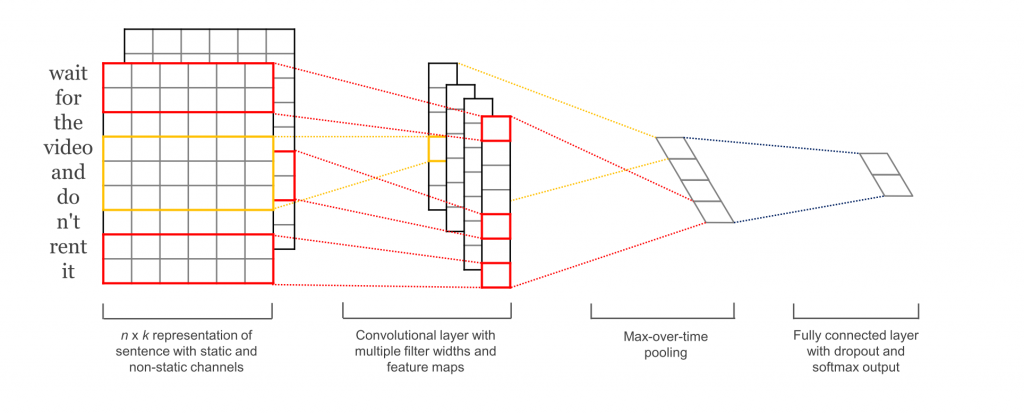
\includegraphics[width=\columnwidth]{cnn.png}
\end{center}
\caption{Image source: ~\cite{Britz}}
\label{fig:figure1}
\end{figure}

We trained different models on all domains (books, dvd, music) and then evaluated them on all the domains. Table ~\ref{cnn-table} gives a summary of the accuracies calculated on test set. Rows mean that a given dataset is evaluated on different models. Columns mean that a given model is evaluated on different data sets. Therefore, for row "books" and column "dvd" means that the model trained on "dvd" is evaluated on "books". As expected, the model performs best when both the training and testing domain is the same. The accuracies are thus the highest across the diagonal. This model uses "ReLU" as the activation and "Adam" as the optimizer.


\begin{table}[h]
\begin{center}
\begin{tabular}{|l|l|l|l|}
\hline \bf & \bf Books & \bf Dvd & \bf Music \\ \hline
Books & 0.766 & 0.7325 & 0.6815 \\
Dvd & 0.7165 & 0.756 & 0.7105 \\
Music & 0.709 & 0.7455 & 0.77 \\
\hline
\end{tabular}
\end{center}
\caption{ Training results for baseline CNN }
\label{cnn-table}
\end{table}



\section{Domain Adversial Training}

Describe the concept.

\subsection{Method}
Describe the specific network.

\subsection{Research Question}

\section{Dataset}
The data is from 3 different domains (books, dvds, movies) and 3 different languages (German, English, French).
We have only used the English dataset for this work. The data has been obtained from: \url{https://www.uni-weimar.de/en/media/chairs/computer-science-and-media/webis/corpora/corpus-webis-cls-10/} and it is described in~\cite{PB:2010}.

For each language and each domain there are 2000 training examples and 2000 test examples. The ratings to positive/negative sentiment are mapped as follows: 1.0, 2.0: negative, 4.0, 5.0: positive. There are no instances with a rating of 3.0. The datasets are balanced, this means for each language and each domain 50\% of the items have a positive and 50\% have a negative rating.

\section{Experiments and Results}

\begin{table}[h]
\begin{center}
\begin{tabular}{|l|l|l|l|l|}
\hline Activation & Domain loss \% & Books & Dvd & Music \\ \hline
Relu & 0.05 & 0.7375 & 0.756 & 0.715  \\
 & 0.1 & 0.741 & 0.7465 & 0.703 \\
 & 0.2 & 0.742 & 0.7435 & 0.7155 \\
\hline
tanh & 0.05 & 0.755 & 0.7655 & 0.7255 \\
 & 0.1 & 0.75 & 0.7515 & 0.7035 \\
 & 0.2 & 0.741 & 0.7355 & 0.7145 \\
\hline
elu & 0.05 & 0.7395 & 0.7515 & 0.712 \\
 & 0.1 & 0.75 & 0.7515 & 0.727 \\
 & 0.2 & 0.7375 & 0.739 & 0.705 \\
\hline
softplus & 0.05 & 0.7545 & 0.766 & 0.7335 \\
 & 0.1 & 0.7585 & 0.763 & 0.747 \\
 & 0.2 & 0.744 & 0.746 & 0.728 \\
\hline
\end{tabular}
\end{center}
\caption{ Training on books-music pair with domain loss factor propagation and activation functions}
\label{dd-table}
\end{table}


\begin{table}[h]
\begin{center}
\begin{tabular}{|l|l|l|l|l|}
\hline Activation & Domain train frequency \% & Books & Dvd & Music \\ \hline
relu & 0.05 & 0.766 & 0.7775 & 0.737 \\
  & 0.1 & 0.7555 & 0.7585 & 0.7185 \\
  & 0.2 & 0.5 & 0.5 & 0.5 \\
\hline
tanh & 0.05 & 0.5 & 0.5 & 0.5  \\
  & 0.1 & 0.754 & 0.767 & 0.719 \\
\hline
elu & 0.05 & 0.755 & 0.7675 & 0.737 \\
  & 0.1 & 0.746 & 0.766 & 0.731 \\
\hline
softplus & 0.05 & 0.766 & 0.7675 & 0.7315 \\
  & 0.1 & 0.76 & 0.768 & 0.721 \\
\hline
\end{tabular}
\end{center}
\caption{ Training on books-music pair with domain train frequency and activation functions}
\label{dd-table}
\end{table}









\section{Conclusion}



% include your own bib file like this:
%\bibliographystyle{acl}
%\bibliography{acl2015}

\begin{thebibliography}{}
% this paper describes the dataset.
\bibitem[\protect\citename{{Prettenhofer and Stein}}2010]{PB:2010}
Prettenhofer, Peter and Stein, Benno
\newblock 2010.
\newblock {\em Cross-language Text Classification Using Structural Correspondence Learning}.
\newblock Proceedings of the 48th Annual Meeting of the Association for Computational Linguistics.

\bibitem[\protect\citename{{Chen \bgroup et al.\egroup }}2016]{Chen:2016}
Xilun Chen and Ben Athiwaratkun and Yu Sun and Kilian Q. Weinberger and Claire Cardie.
\newblock 2016.
\newblock {\em Adversarial Deep Averaging Networks for Cross-Lingual Sentiment Classification}.
\newblock CoRR.

\bibitem[\protect\citename{{Ganin \bgroup et al.\egroup }}2016]{Ganin:2016}
Ganin, Yaroslav and Ustinova, Evgeniya and Ajakan, Hana and Germain, Pascal and Larochelle, Hugo and Laviolette, Fran\c{c}ois and Marchand, Mario and Lempitsky, Victor.
\newblock 2016.
\newblock {\em Domain-adversarial Training of Neural Networks},
  17(1):2096--2030.
\newblock J. Mach. Learn. Res.

\bibitem[\protect\citename{{Britz}}2015]{Britz}
Denny Britz.
\newblock 2015.
\newblock {\em Implementing a CNN for Text Classification in TensorFlow}.
\newblock http://www.wildml.com/2015/12/implementing-a-cnn-for-text-classification-in-tensorflow/.

\bibitem[\protect\citename{{Britz Github}}2015]{Britz:github}
Denny Britz.
\newblock 2015.
\newblock {\em dennybritz/cnn-text-classification-tf}.
\newblock https://github.com/dennybritz/cnn-text-classification-tf.


\end{thebibliography}

\end{document}
